\documentclass[12pt]{article}

% You need graphics package
\usepackage{color}
\usepackage{graphicx}
\usepackage{pst-all}
\usepackage[annot]{../tex/advi}
\pagestyle{empty}

\definecolor{red}{rgb}{1.0,0.8,0.8}
\definecolor{green}{rgb}{0.8,1.0,0.8}
\definecolor{blue}{rgb}{0.8,0.8,1.0}
\definecolor{yellow}{rgb}{1.0,1.0,0.8}
\definecolor{magenta}{rgb}{1.0,0.8,1.0}
\definecolor{cyan}{rgb}{0.8,1.0,1.0}

\def\smallpause{0.3}

\def\advifooter{\vbox to 0em{\vbox to \vsize {\vfill
Press: \underline{n}ext page \underline{p}revious page
\underline{\textvisiblespace} next pause} \vss}}

\def\adviheader{\noindent
{\bf\Large Active dvi --- transitions}\\

\includegraphics[width=\textwidth]{../tex/bar.jpg.eps}}

\def\adviback#1{%
\hspace{-\textwidth}
\rput(-0.7cm,-0.5cm){\psframe[framearc=.1,fillstyle=solid,linestyle=none,fillcolor=#1](1.1\textwidth,-0.85\textheight)}
}

\let\Newpage\newpage
\def\newpage{\Newpage\advifooter\adviheader}

\def\adviemptyfooter{\vbox to 0em{\vbox to \vsize {\vfill
~~} \vss}}

\def\lastpage{\Newpage\adviemptyfooter\adviheader}

%  \setlength\textwidth{660\p@}
%  \setlength\textheight{460\p@}

\begin{document}
 
\newpage\adviback{red}

\subsection* {Transitions}
Active dvi has transitions --- animated page display for each pause.
You can specify the transition by \verb|\settransition{|%
$mode~arg_1~\ldots~arg_n$\verb|}| advi macro.
Currently the following transition modes are available:
\begin{itemize}
\item {\tt none } --- no transition animation  
\item {\tt slide}  --- new page slides on the screen
\item {\tt wipe } --- new page wipes on the screen
\item {\tt block}  --- new page is split into small pieces and 
  they appear randomly
\end{itemize}
For example, if you want to slide the page, write
\verb+\settransition{slide}+ in your document. 

\subsection*{Notes}
\begin{itemize}
\item The transition state of advi is currently reset to \verb|none|
  at the beginning of each page.
\item The transition animations occur even at \verb+\pause+ and
  \verb+\wait+ commands. 
  If you feel it too lousy for each pause, 
  you have to disable the transition by \verb+\settransition{none}+
  just before pauses.
\end{itemize}

\newpage\adviback{green}

\subsection* {Transitions parameters}
Each transition mode has additional parameters to control its details. 
Usually the followings are available:
\begin{itemize}
\item {\tt from=}{\em{arg}} --- new pages come from the direction of
  {\em arg} (\verb+left+, \verb+top+, \verb+topleft+, etc) 
\item {\tt steps=}{\em{arg}}  --- animation steps
\end{itemize}
For example, if you want to slide-in a page from left in 30 steps,
write \verb+\settransition{slide from=left steps=30}+.

\newpage\adviback{blue}

\subsection* {Slide transition}
\settransition{slide from=left steps=30}
New pages appears sliding into the screen.

\subsubsection*{Options}
\begin{itemize}
\item {\tt from=}{\em{arg}} --- new pages come from the direction of
  {\em arg} (one of \verb+left+, \verb+right+, \verb+top+,
  \verb+bottom+, \verb+topleft+, \verb+topright+, \verb+bottomleft+,
  \verb+bottomright+). The default is \verb+right+.
\item {\tt steps=}{\em{arg}}  --- animation steps. The default is \verb+20+.
\end{itemize}

\subsubsection*{Examples}
\begin{itemize}
\item \verb+\settransition{slide}+
\item \verb+\settransition{slide from=left steps=30}+
\end{itemize}

\newpage\adviback{yellow}
\settransition{wipe from=right steps=30}

\subsection* {Wipe transition}
New pages appears wiping out the old graphics.

\subsubsection*{Options}
\begin{itemize}
\item {\tt from=}{\em{arg}} --- new pages come from the direction of
  {\em arg} (one of \verb+left+, \verb+right+, \verb+top+,
  \verb+bottom+, \verb+topleft+, \verb+topright+, \verb+bottomleft+,
  \verb+bottomright+, \verb+center+). The default is \verb+right+.
\item {\tt steps=}{\em{arg}}  --- animation steps. The default is \verb+20+.
\end{itemize}

\subsubsection*{Examples}
\begin{itemize}
\item \verb+\settransition{wipe}+
\item \verb+\settransition{wipe from=center steps=30}+
\end{itemize}

\newpage\adviback{magenta}
\settransition{block from=topleft steps=20000}

\subsection* {Block transition}
New pages appears gradually into small pieces.

\subsubsection*{Options}
\begin{itemize}
\item {\tt from=}{\em{arg}} --- new pages come from the direction of
  {\em arg} (one of \verb+left+, \verb+right+, \verb+top+,
  \verb+bottom+, \verb+topleft+, \verb+topright+, \verb+bottomleft+,
  \verb+bottomright+, \verb+center+). The default is \verb+right+.
\item {\tt steps=}{\em{arg}}  --- number of blocks. The default is \verb+5000+.
\end{itemize}

\subsubsection*{Examples}
\begin{itemize}
\item \verb+\settransition{block}+
\item \verb+\settransition{block from=topleft steps=10000}+
\end{itemize}

\lastpage

~\vfill
\begin{center}
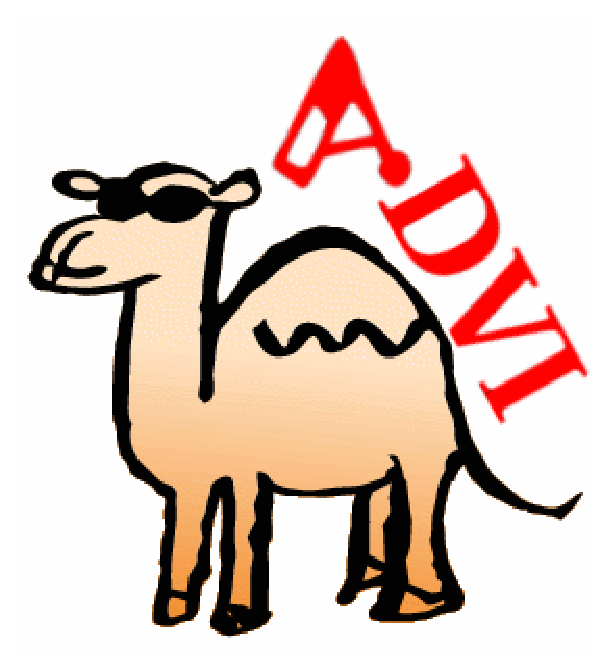
\includegraphics[width=0.5\textwidth]{../tex/advilogo.eps}\\
{\Large \bf That's all, folks!!}
\end{center}
\vfill

\end{document}
